% Title:
% 	Corporate presentation template
% ----------------------
% Description:
% 	A presentation template which does not look too academic.
%
% Creator: Tommy O.

% -------------------------------------------------------------------------
% Setup
% -------------------------------------------------------------------------
\documentclass[12pt, aspectratio=149]{beamer}
% Options for aspectratio: 1610, 149, 54, 43 and 32, 169
\usepackage[utf8]{inputenc}
\usepackage[norsk]{babel}% Alternative: 'norsk'
\usepackage[expansion=false]{microtype}% Fixes to make typography better
\usecolortheme{beaver} % Decent options: beaver, rose, crane
%\useoutertheme{split}
%\useoutertheme[footline=authortitle]{miniframes}
\usepackage{txfonts}% Font which looks less 'academic'
\usepackage{listings}% To include source-code
\usepackage{booktabs}% Professional tables
\usefonttheme{serif}
\usepackage{mathptmx}
\usepackage[scaled=0.9]{helvet}
\usepackage{courier}


\title{An introduction to probabilistic programming with PyMC3}
%\subtitle{Presentation subtitle}
\institute{
\includegraphics[width=.1\textwidth]{figs/inmeta.png}}
%\titlegraphic{
\includegraphics[width=.1\textwidth]{figs/inmeta.png}}
\date[fontsize=\tiny]{\today}
\author{Sean Meling Murray and Solveig Masvie}

% -------------------------------------------------------------------------
% Package imports
% -------------------------------------------------------------------------
\usepackage{etoolbox}
\usepackage{graphicx}
\usepackage{tikz}
\usepackage{amsmath}
\usepackage{amsthm}
\usepackage{amsfonts}
\usepackage{amssymb}
\usepackage{mathtools}
\usepackage{graphicx}
\usepackage{hyperref}
\usepackage{listings}
\usepackage[sharp]{easylist}
\usepackage{multicol}
\usepackage{tikz-cd}
\usepackage{xcolor}
\usepackage{algorithm2e}
\usepackage{algorithmic}
\usepackage{float}
\usepackage{listings}
\usepackage{minted}

%gets rid of bottom navigation bars
\setbeamertemplate{footline}[frame number]{}

%gets rid of bottom navigation symbols
\setbeamertemplate{navigation symbols}{}

% Set up colors to be used
\definecolor{purered}{RGB}{204,0,0}
\definecolor{titlered}{RGB}{148,0,211}
\definecolor{bggray}{RGB}{242,242,242}
\definecolor{bggraydark}{RGB}{217,217,217}

% Change the default colors

\setbeamercolor*{title}{bg=bggray,fg=titlered}
\AtBeginEnvironment{theorem}{%
	\setbeamercolor{block title}{fg=titlered, bg=bggraydark}
	\setbeamercolor{block body}{fg=black,bg=bggray}
}
\AtBeginEnvironment{proof}{%
	\setbeamercolor{block title}{bg=bggraydark}
	\setbeamercolor{block body}{fg=black,bg=bggray}
}
\AtBeginEnvironment{example}{%
	\setbeamercolor{block title example}{bg=bggraydark}
	\setbeamercolor{block body example}{fg=black,bg=bggray}
}
\AtBeginEnvironment{definition}{%
	\setbeamercolor{block title}{bg=bggraydark}
	\setbeamercolor{block body}{fg=black,bg=bggray}
}

\setbeamercolor{block title example}{bg=bggraydark}
\setbeamercolor{block body example}{fg=black,bg=bggray}
\setbeamercolor{block title}{bg=bggraydark}
\setbeamercolor{block body}{fg=black,bg=bggray}

\setbeamercolor{frametitle}{fg=titlered,bg=bggray}
\setbeamercolor{section in head/foot}{bg=black}
\setbeamercolor{author in head/foot}{bg=black}
\setbeamercolor{date in head/foot}{fg=titlered}

% Spacing for lsits
\newcommand{\listSpace}{0.2em}

% Theorems, equations, definitions setup
\theoremstyle{plain}

% -------------------------------------------------------------------------
% Document start
% -------------------------------------------------------------------------
\begin{document}
\maketitle
\addtobeamertemplate{frametitle}{}{%
\begin{tikzpicture}[remember picture,overlay]
  	\node[anchor=south west,yshift=0pt, xshift=4pt, scale=0.7] at (current page.south west) {
\includegraphics[height=0.3cm]{figs/inmeta.png}};
\end{tikzpicture}}

% -------------------------------------------------------------------------
\section{Introduction}
\begin{frame}[fragile]{Road map}
	\begin{easylist}[enumerate]
		\ListProperties(Space=\listSpace, Margin1=1ex, Margin2=2ex, Space*=\listSpace)
		# Theory
		## The basics of Bayesianism
		## Markov chain Monte Carlo methods (MCMC)
		# Practice
		## Probabilistic programming with PyMC3
	\end{easylist}
\end{frame}

\begin{frame}[fragile]{What is Bayesian data analysis?}
	\begin{columns}
		\begin{column}{0.7\linewidth}
			``A Bayesian is one who, vaguely expecting a horse, and catching a glimpse of a donkey, strongly believes he has seen a mule.''
		\end{column}
		\begin{column}{0.3\linewidth}
			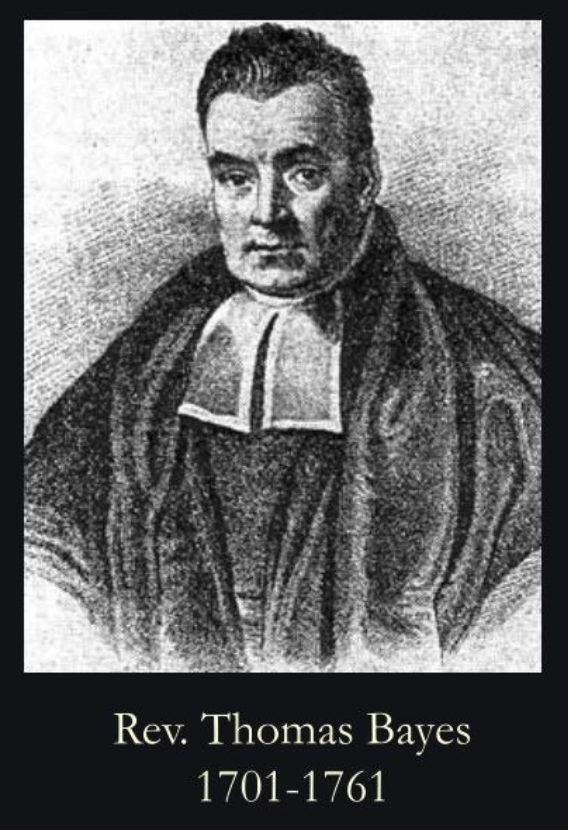
\includegraphics[height=0.7\textheight]{figs/bayes.png}
		\end{column}
	\end{columns}
\end{frame}

\begin{frame}[fragile]{It's just counting!}
	\begin{columns}
		\begin{column}{0.7\linewidth}
			\begin{easylist}[itemize]
					\ListProperties(Space=\listSpace, Margin1=1ex, Space*=\listSpace)
					# Richard McElreath: ``Bayesian inference is just counting.''  
					# Count all the ways observed data could have arisen according to assumptions
					# Assumptions that can arise in more ways are more consistent with the data, and therefore more plausible
			\end{easylist}
		\end{column}
	\begin{column}{0.3\textwidth}
		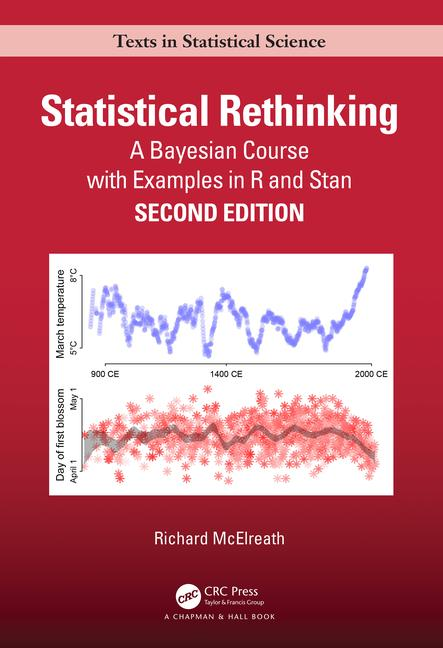
\includegraphics[height=0.7\textheight]{figs/rethinking3.jpg}
	\end{column}
	\end{columns}
\end{frame}

\begin{frame}[fragile]{The Garden of Forking Data}
	\begin{center}
		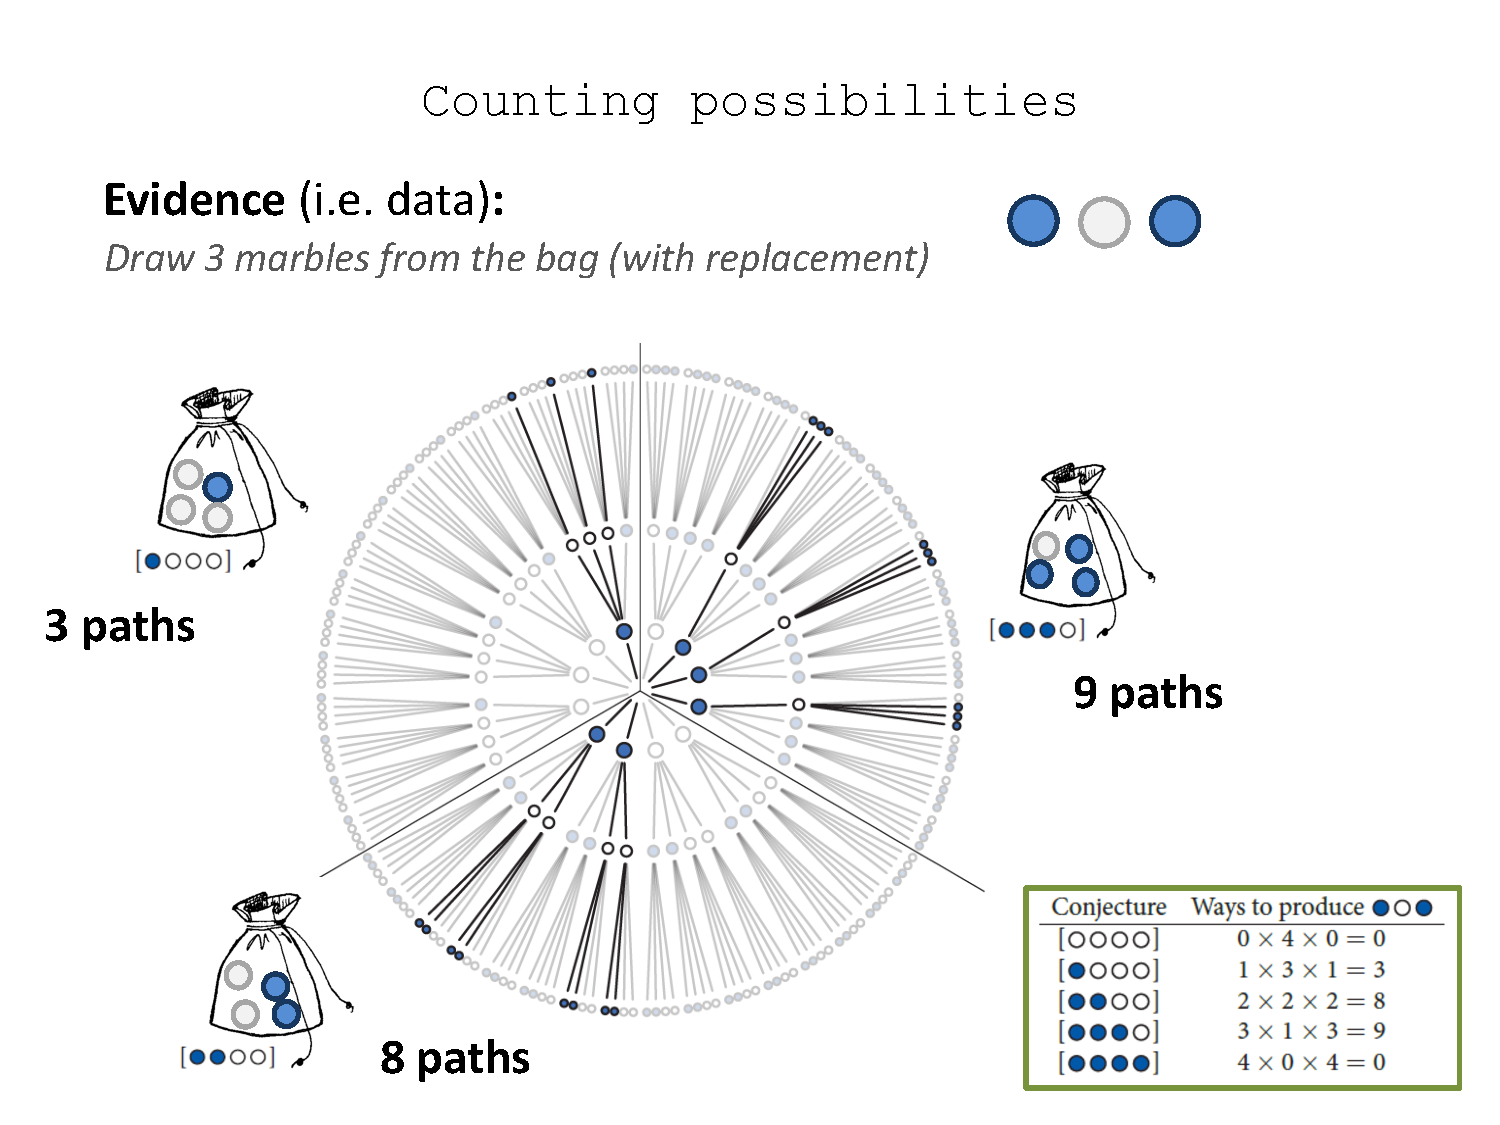
\includegraphics[height=0.8\textheight]{figs/forkingpaths.pdf}
	\end{center}
\end{frame}

\begin{frame}[fragile]{Priors, posteriors and likelihoods}
	\begin{columns}
		\begin{column}{0.5\linewidth}
			Prior $p(\theta)$: Encodes assumptions about $\theta$\\
			Likelihood $p(y \, \vert \, \theta)$: How were the observed data generated? \\ 
			Posterior $p(\theta \, \vert \, y)$: Assumptions about $\theta$ consistent with data
			\begin{equation*}
			\begin{split}
			p(\theta \vert \, y) & =  \frac{p(\theta)p(y \, \vert \theta)}{\int p(y \, \vert \theta)p(\theta) \, d\theta} \\
			& \propto p(\theta)p(y \, \vert \theta)
			\end{split}
			\end{equation*}
			\begin{equation*}
			\textcolor{red}{posterior} \propto  \textcolor{orange}{prior} \cdot \textcolor{blue}{likelihood}
			\end{equation*}
		\end{column}
		\begin{column}{0.5\linewidth}
			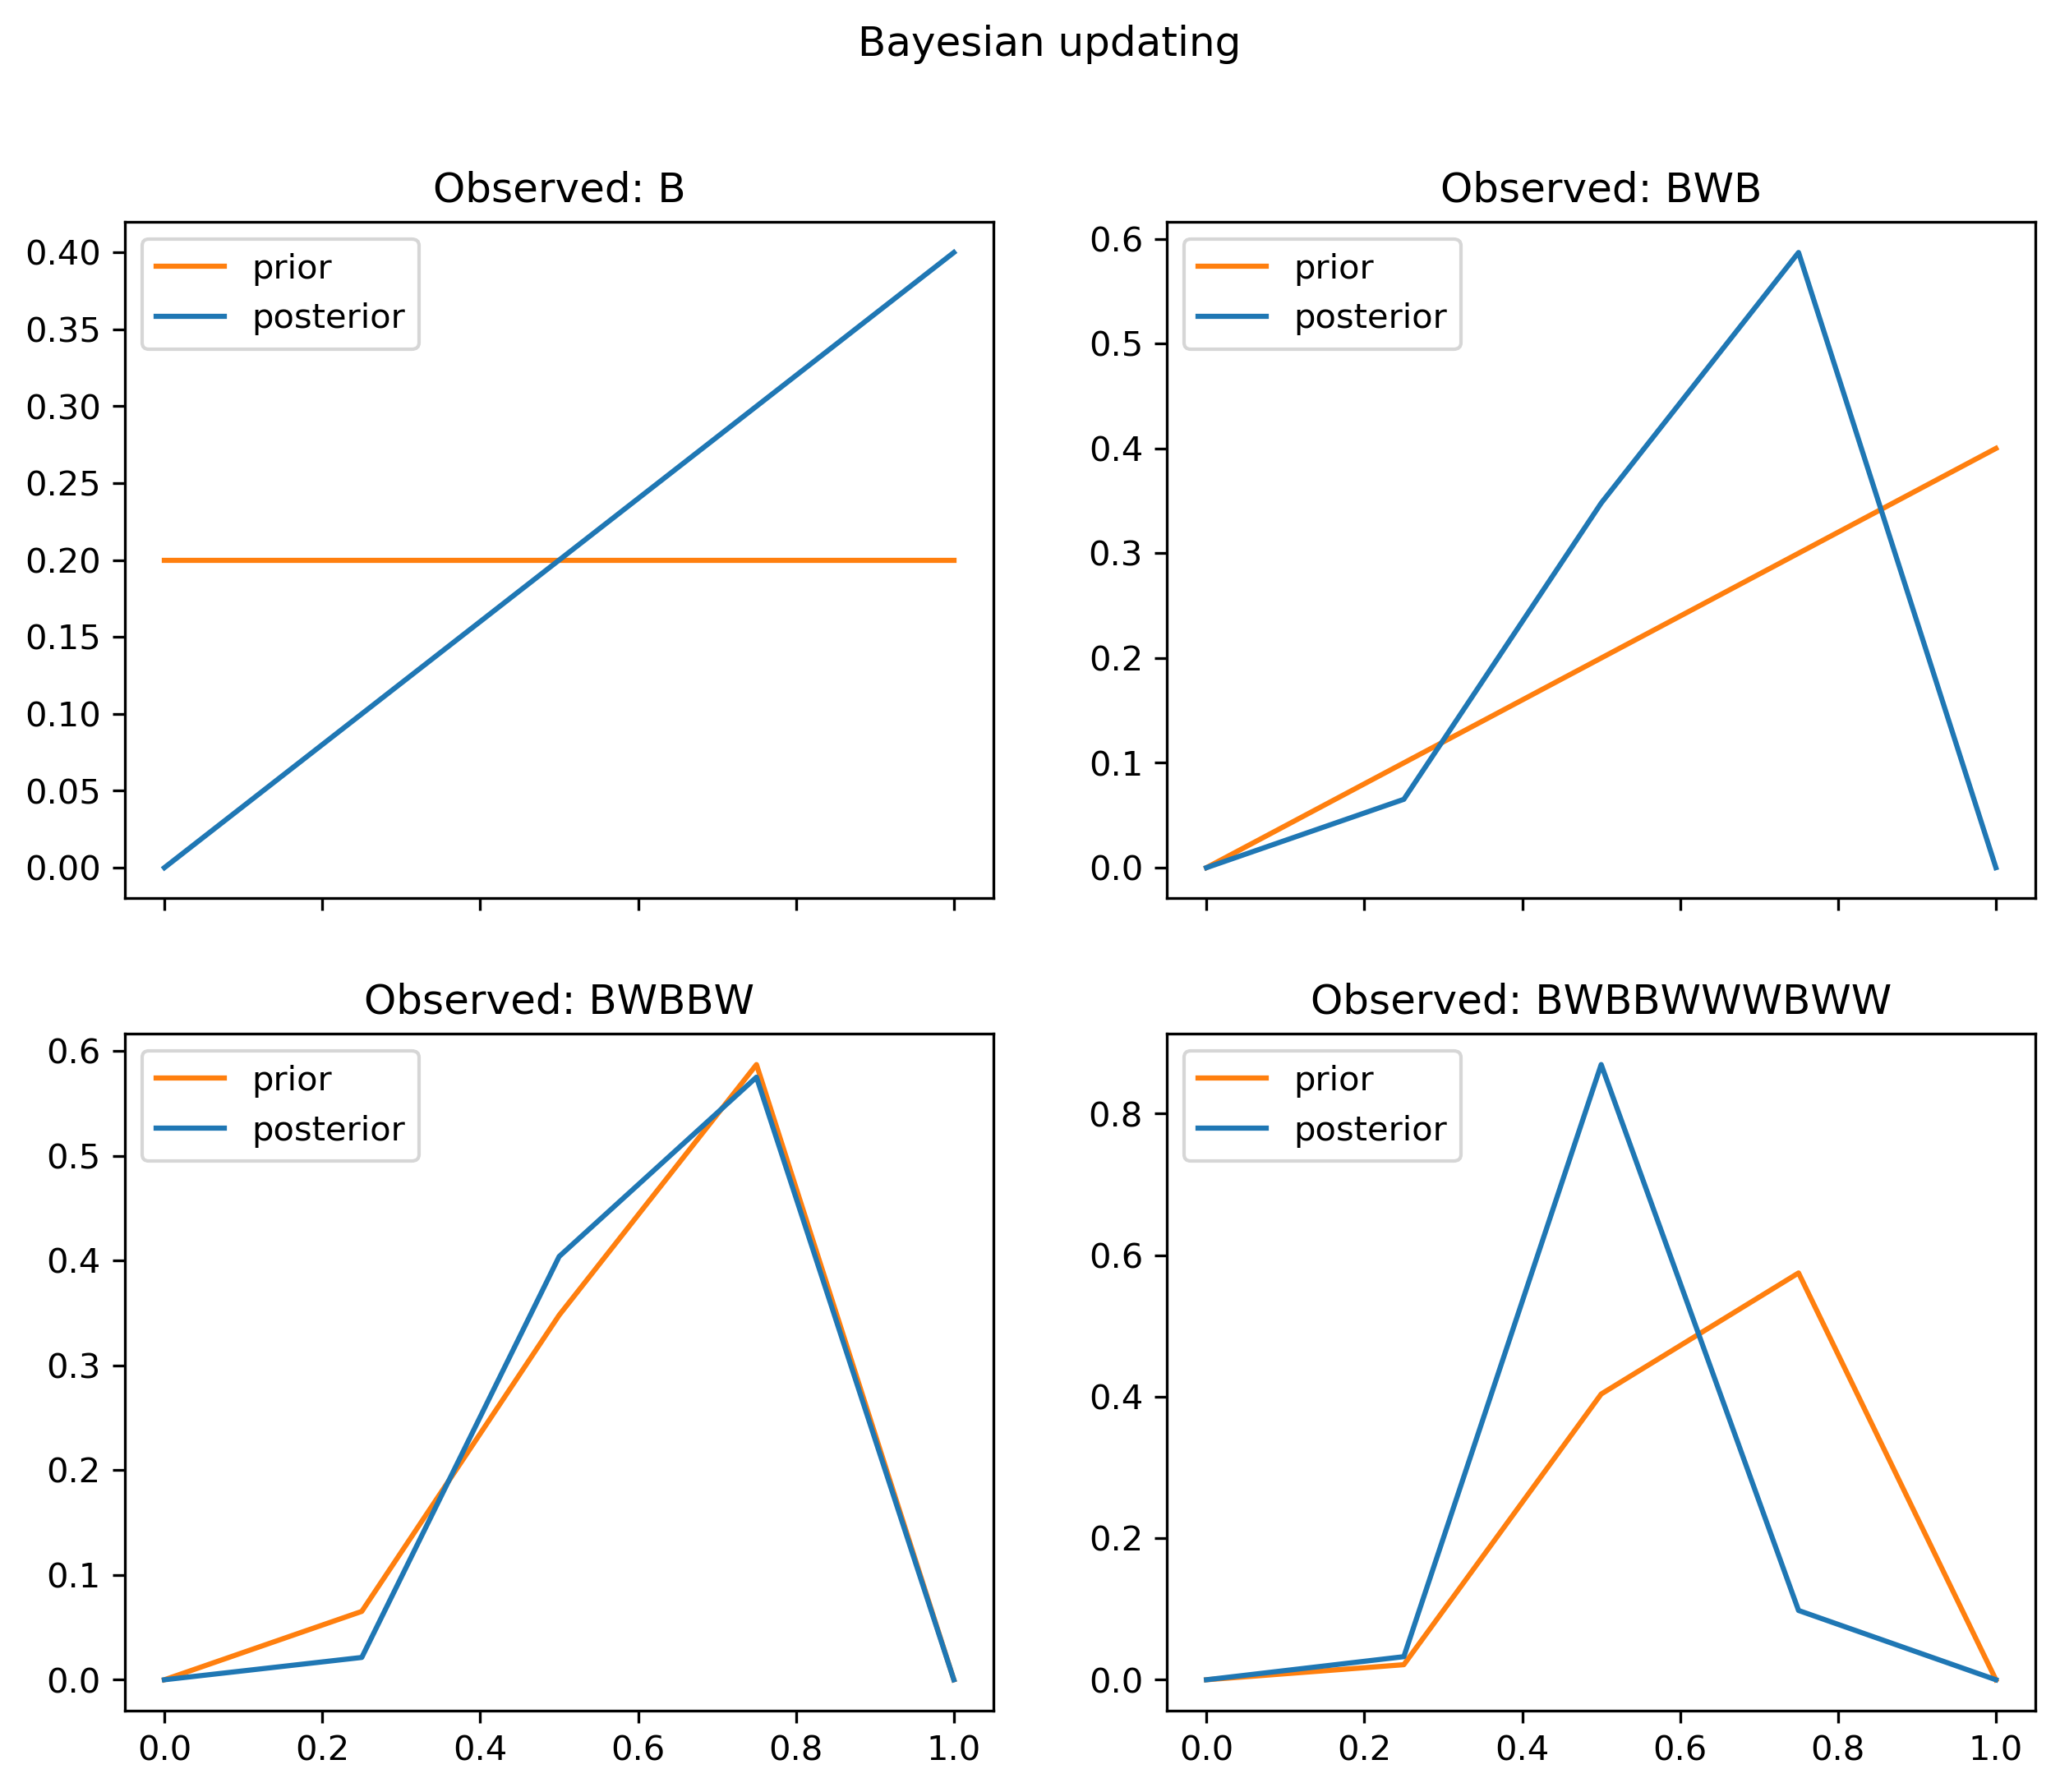
\includegraphics[scale=0.3]{figs/updating.png}
		\end{column}
	\end{columns}
\end{frame}

\begin{frame}[fragile]{Towards a Bayesian workflow}
	\begin{easylist}[enumerate]
		\ListProperties(Space=\listSpace, Margin1=1ex, Margin2=2ex, Space*=\listSpace)
		# Design the model (tell the data story)
		## Describe data generating process: $p(y \, \vert \theta) = \theta^{blue} (1 - \theta)^{white}$
		## Encode assumptions about parameters: $p(\theta) = \frac{1}{5}$
		# Condition on the data (update step)
		## $p(\theta \vert \, y) \propto p(\theta) p(y \, \vert \theta)$
		# Evaluate the model (critique), and either
		## be happy, it worked as planned, or
		## return to step 1
	\end{easylist}
\end{frame}

\begin{frame}[fragile]{The Garden of Forking Data, revisited}
	\inputminted[fontsize=\tiny]{python}{../code/marbles.py}
\end{frame}

\begin{frame}[fragile]{The Garden of Forking Data, revisited}
	\inputminted[fontsize=\tiny]{python}{../code/forking_data.py}
\end{frame}

\begin{frame}[fragile]{The Frequentist vs. Bayesian debacle}
	\begin{columns}
		\begin{column}{0.7\linewidth}
			\begin{easylist}[itemize]
				\ListProperties(Space=\listSpace, Margin1=1ex, Margin2=2ex, Space*=\listSpace, Style2*=$\color{bggraydark}\blacktriangleright$\space)
				# Frequentist statistics
				## Probability $=$ limiting frequency
				## Uncertainty arises from sampling variation
				# Bayesian statistics
				## Frequency $\neq$ probability
				## Uncertainty arises from ignorance
				# Principled way to represent and take into account uncertainty
				# Easily incorporates prior information
			\end{easylist}
		\end{column}
		\begin{column}{0.3\textwidth}
			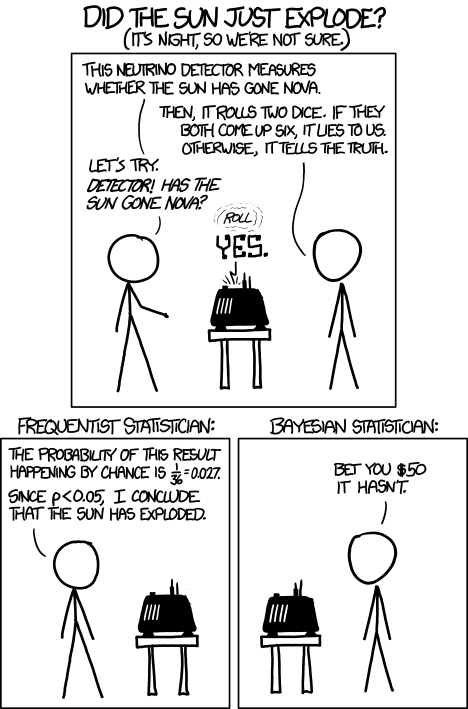
\includegraphics[height=0.7\textheight]{figs/relevant_xkcd.png}
		\end{column}
	\end{columns}
\end{frame}

\begin{frame}[fragile]{But priors are subjective! Buu! Hiss!}
	\begin{easylist}
		\ListProperties(Space=\listSpace, Margin1=1ex, Margin2=2ex, Space*=\listSpace, Style2*=$\color{bggraydark}\blacktriangleright$\space)
		# Non-informative vs. informative priors
		## Forking data example: $Uniform(0, 1)$ vs. $Uniform(\frac{1}{4}, \frac{3}{4})$
		# Test your assumptions, e.g. using prior predictive checks
		# More about priors:
		## Gelman et al. (2017): \footnotesize\texttt{https://arxiv.org/abs/1708.07487}
		## Bayesian Methods for Hackers: \footnotesize\texttt{https://tinyurl.com/v2yzyqv}	
		# For more Bayesian challenges, see e.g. Gelman and Yao (2020): \footnotesize\texttt{https://tinyurl.com/sbr2tev}
	\end{easylist}
\end{frame}

\begin{frame}[fragile]{Telling the data story}
	`` People think in terms of stories - thus the unreasonable power of the anecdote to drive decision-making, well-founded or not. Existing analytics largely fails to provide this kind of story; instead, numbers seemingly appear out of thin air.'' \\
	\flushright Beau Cronin, \textit{Why Probabilistic Programming Matters (2013)}
\end{frame}

\begin{frame}[fragile]{How to sample from intractable posteriors?}
	\begin{columns}
		\begin{column}{0.5\linewidth}
		\begin{easylist}
			\ListProperties(Space=\listSpace, Margin1=1ex, Margin2=2ex, Space*=\listSpace, Style2*=$\color{bggraydark}\blacktriangleright$\space)
			# In textbooks, nice, we can sample directly from well-behaved, analytical posteriors
			# In the real world, often impossible to sample directly from $p(\theta \vert y)$
			# A general class of algorithms called \textbf{Markov chain Monte Carlo} let us approximately sample from posterior
		\end{easylist}		
		\end{column}
		\begin{column}{0.5\linewidth}
		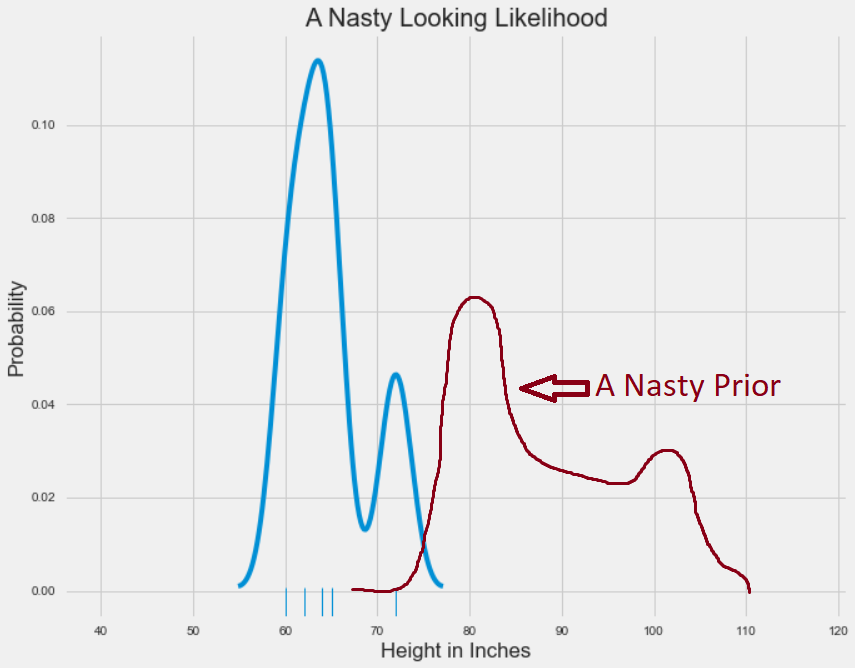
\includegraphics[scale=0.2]{figs/nasty_prior_posterior_example.png}
		\end{column}
	\end{columns}
\end{frame}

\begin{frame}[fragile]{Markov chains}
	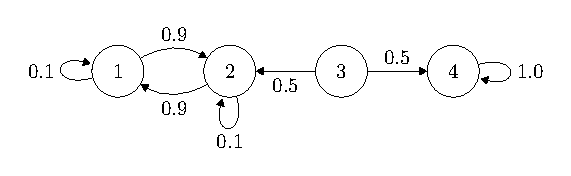
\includegraphics[scale=.8]{figs/irreducible.pdf}
	\begin{easylist}[itemize]
		\ListProperties(Space=\listSpace, Margin1=1ex, Margin2=2ex, Space*=\listSpace, Style2*=$\color{bggraydark}\blacktriangleright$\space)
		# A Markov chain defines a joint probability distribution over sequences
		# Used to model events in discrete and continuous time (manufacturing processes, queuing systems, etc.)
		# Typically interested in the long-term distribution of being in a certain state
	\end{easylist}
\end{frame}

\begin{frame}[fragile]{Properties of a Markov chain}
	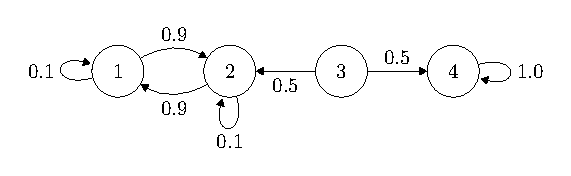
\includegraphics[scale=.8]{figs/irreducible.pdf}
	\begin{easylist}
		\ListProperties(Space=\listSpace, Margin1=1ex, Margin2=2ex, Space*=\listSpace, Style2*=$\color{bggraydark}\blacktriangleright$\space)
		# Memoryless (Markov property): $P(X_t\,|\,X_{t-1}, X_{t-2}, \ldots, X_1) = P(X_t\,|\,X_{t-1})$
		# Under certain conditions, guaranteed to have a unique, limiting distribution (aka. stationary distribution)
		## Long run proportion of time spent in each state
		## For more details, check \footnotesize\texttt{https://github.com/smu095/presentations/}
	\end{easylist}
\end{frame}

\begin{frame}[fragile]{Monte Carlo simulations}
	\begin{easylist}
		\ListProperties(Space=\listSpace, Margin1=1ex, Margin2=2ex, Space*=\listSpace, Style2*=$\color{bggraydark}\blacktriangleright$\space)
		# Monte Carlo (MC) simulations are just a way to approximate numerical results using repeated random sampling
		# Main idea:
		## Generate $N$ samples $x_1, \ldots, x_N$ from $p(x)$, approximate $f$ using the empirical distribution of $\{f(x_n)\}_{n=1}^N$
		## $\mathbb{E}\left[ \, f \, \right] = \int f(x)p(x) \,dx \approx \frac{1}{N} \sum_{n=1}^{N} f(x_n) = \hat{f}$ 
		# MC estimates converge thanks to Law of Large Numbers
		## $(\hat{f} - \mathbb{E}\left[ \, f \, \right]) \rightarrow \mathcal{N}\Big(0, \frac{Var\left[\,f\,\right]}{N_{eff}}\Big)$ as $N \rightarrow \infty$
	\end{easylist}
\end{frame}

\begin{frame}[fragile]{Application: Evaluate integrals}
	\begin{easylist}
		\ListProperties(Space=\listSpace, Margin1=1ex, Margin2=2ex, Space*=\listSpace, Style2*=$\color{bggraydark}\blacktriangleright$\space)
		# Calculate difficult integrals, such as the area of the Batman sign
	\end{easylist}
	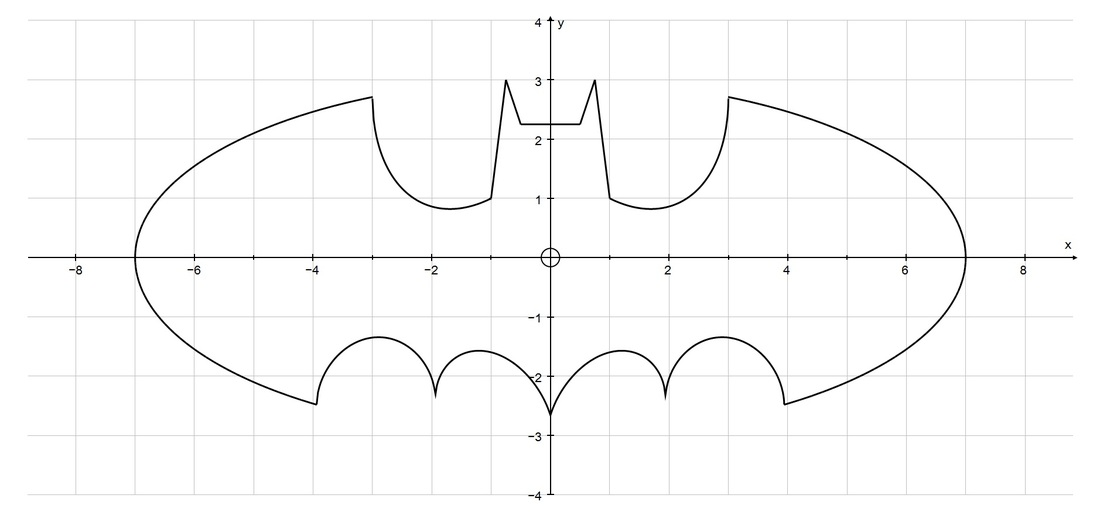
\includegraphics[scale=0.3]{figs/bat_signal.png}
\end{frame}
%https://towardsdatascience.com/a-zero-math-introduction-to-markov-chain-monte-carlo-methods-dcba889e0c50

\begin{frame}[fragile]{Application: Evaluate integrals}
	\begin{easylist}
		\ListProperties(Space=\listSpace, Margin1=1ex, Margin2=2ex, Space*=\listSpace, Style2*=$\color{bggraydark}\blacktriangleright$\space)
		# Repeatedly sample $(u_1, u_2) \sim \text{Uniform}(-\frac{1}{2}, \frac{1}{2})$
		# Calculate area $A$ of Batman sign as $A = \textrm{area of rectangle} \times \frac{\textrm{green dots}}{\textrm{all dots}}$
	\end{easylist}
	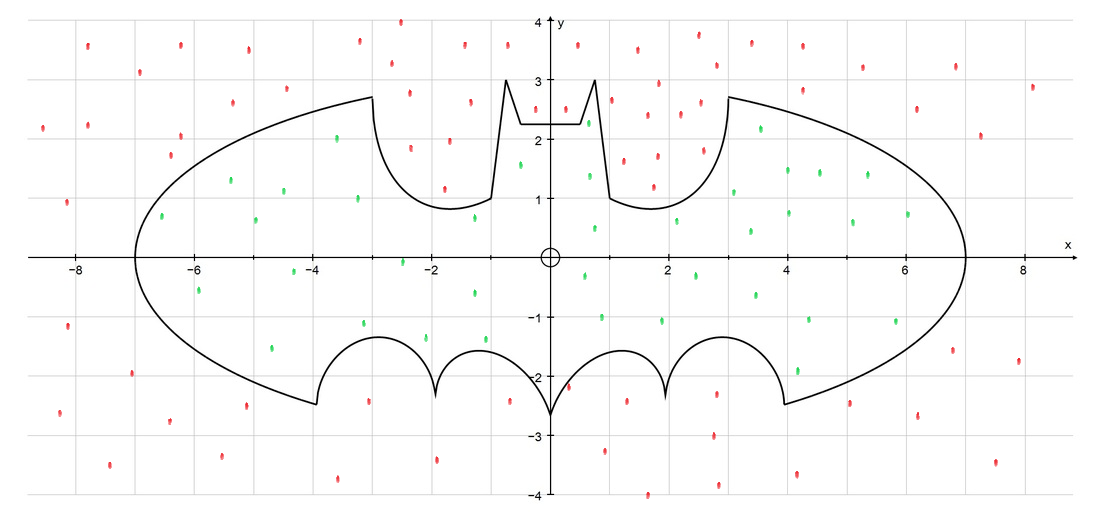
\includegraphics[scale=0.3]{figs/bat_signal_mcs.png}
\end{frame}

\begin{frame}[fragile]{Markov chain Monte Carlo methods}
	\begin{easylist}
		\ListProperties(Space=\listSpace, Margin1=1ex, Margin2=2ex, Space*=\listSpace, Style2*=$\color{bggraydark}\blacktriangleright$\space)
		# \textbf{Main idea:} Construct a Markov chain over the parameter space where the stationary distribution is the posterior $p(\theta \,\vert\, y)$
		## For more details, check \footnotesize\texttt{https://github.com/smu095/presentations/}
		# Randomly move around the parameter space such that the fraction of time spent at each randomly sampled parameter value is proportional to the true target density $p(\theta \,\vert\,y)$.
		# Use the sequence of parameters generated by Markov chain to calculate MC approximations of any quantity of interest
	\end{easylist}
\end{frame}

\begin{frame}[fragile]{Algorithmic view of MCMC}
	\begin{easylist}[enumerate]
		\ListProperties(Space=\listSpace, Margin1=1ex, Margin2=2ex, Space*=\listSpace)
		# Start at current position.
		# Propose new position.
		# Accept/reject new position based on position's adherence to data and prior distributions.
		## If reject: Remain in your current position, return to step 1.
		## If accept: Move to the new position, return to step 1.
		# After large number of iterations, return sequence of accepted positions.
	\end{easylist}
\end{frame}

\begin{frame}[fragile]{Metropolis algorithm}
	\begin{easylist}[enumerate]
		\ListProperties(Space=\listSpace, Margin1=1ex, Margin2=2ex, Space*=\listSpace)
		# Start at some initial parameter value $\theta_0$
		# for $t=1$ to $T$:
		## Sample $\theta^*$ from a proposal distribution $q(\theta^* \, \vert \, \theta_{t-1})$
		## Evaluate $\alpha_{\theta^*}= \dfrac{p(\theta^* \, \vert \, y)}{p(\theta_{t-1} \, \vert \, y)}$.\\
		## Set acceptance probability to $r_{\theta^*}= \text{min}(1, \alpha_{\theta^*})$.\\
		## Draw $u \sim Uniform(0, 1)$
		## Set $\theta_t = \begin{cases}\theta^*, &\text{if}\ u < r \\ \theta_{t-1}, &\text{o.w.}\ \end{cases}$
	\end{easylist}
\end{frame}

\begin{frame}[fragile]{Metropolis in Python}
	\inputminted[fontsize=\tiny]{python}{../code/metropolis.py}
\end{frame}

\begin{frame}[fragile]{Metropolis in Python}
	\center
	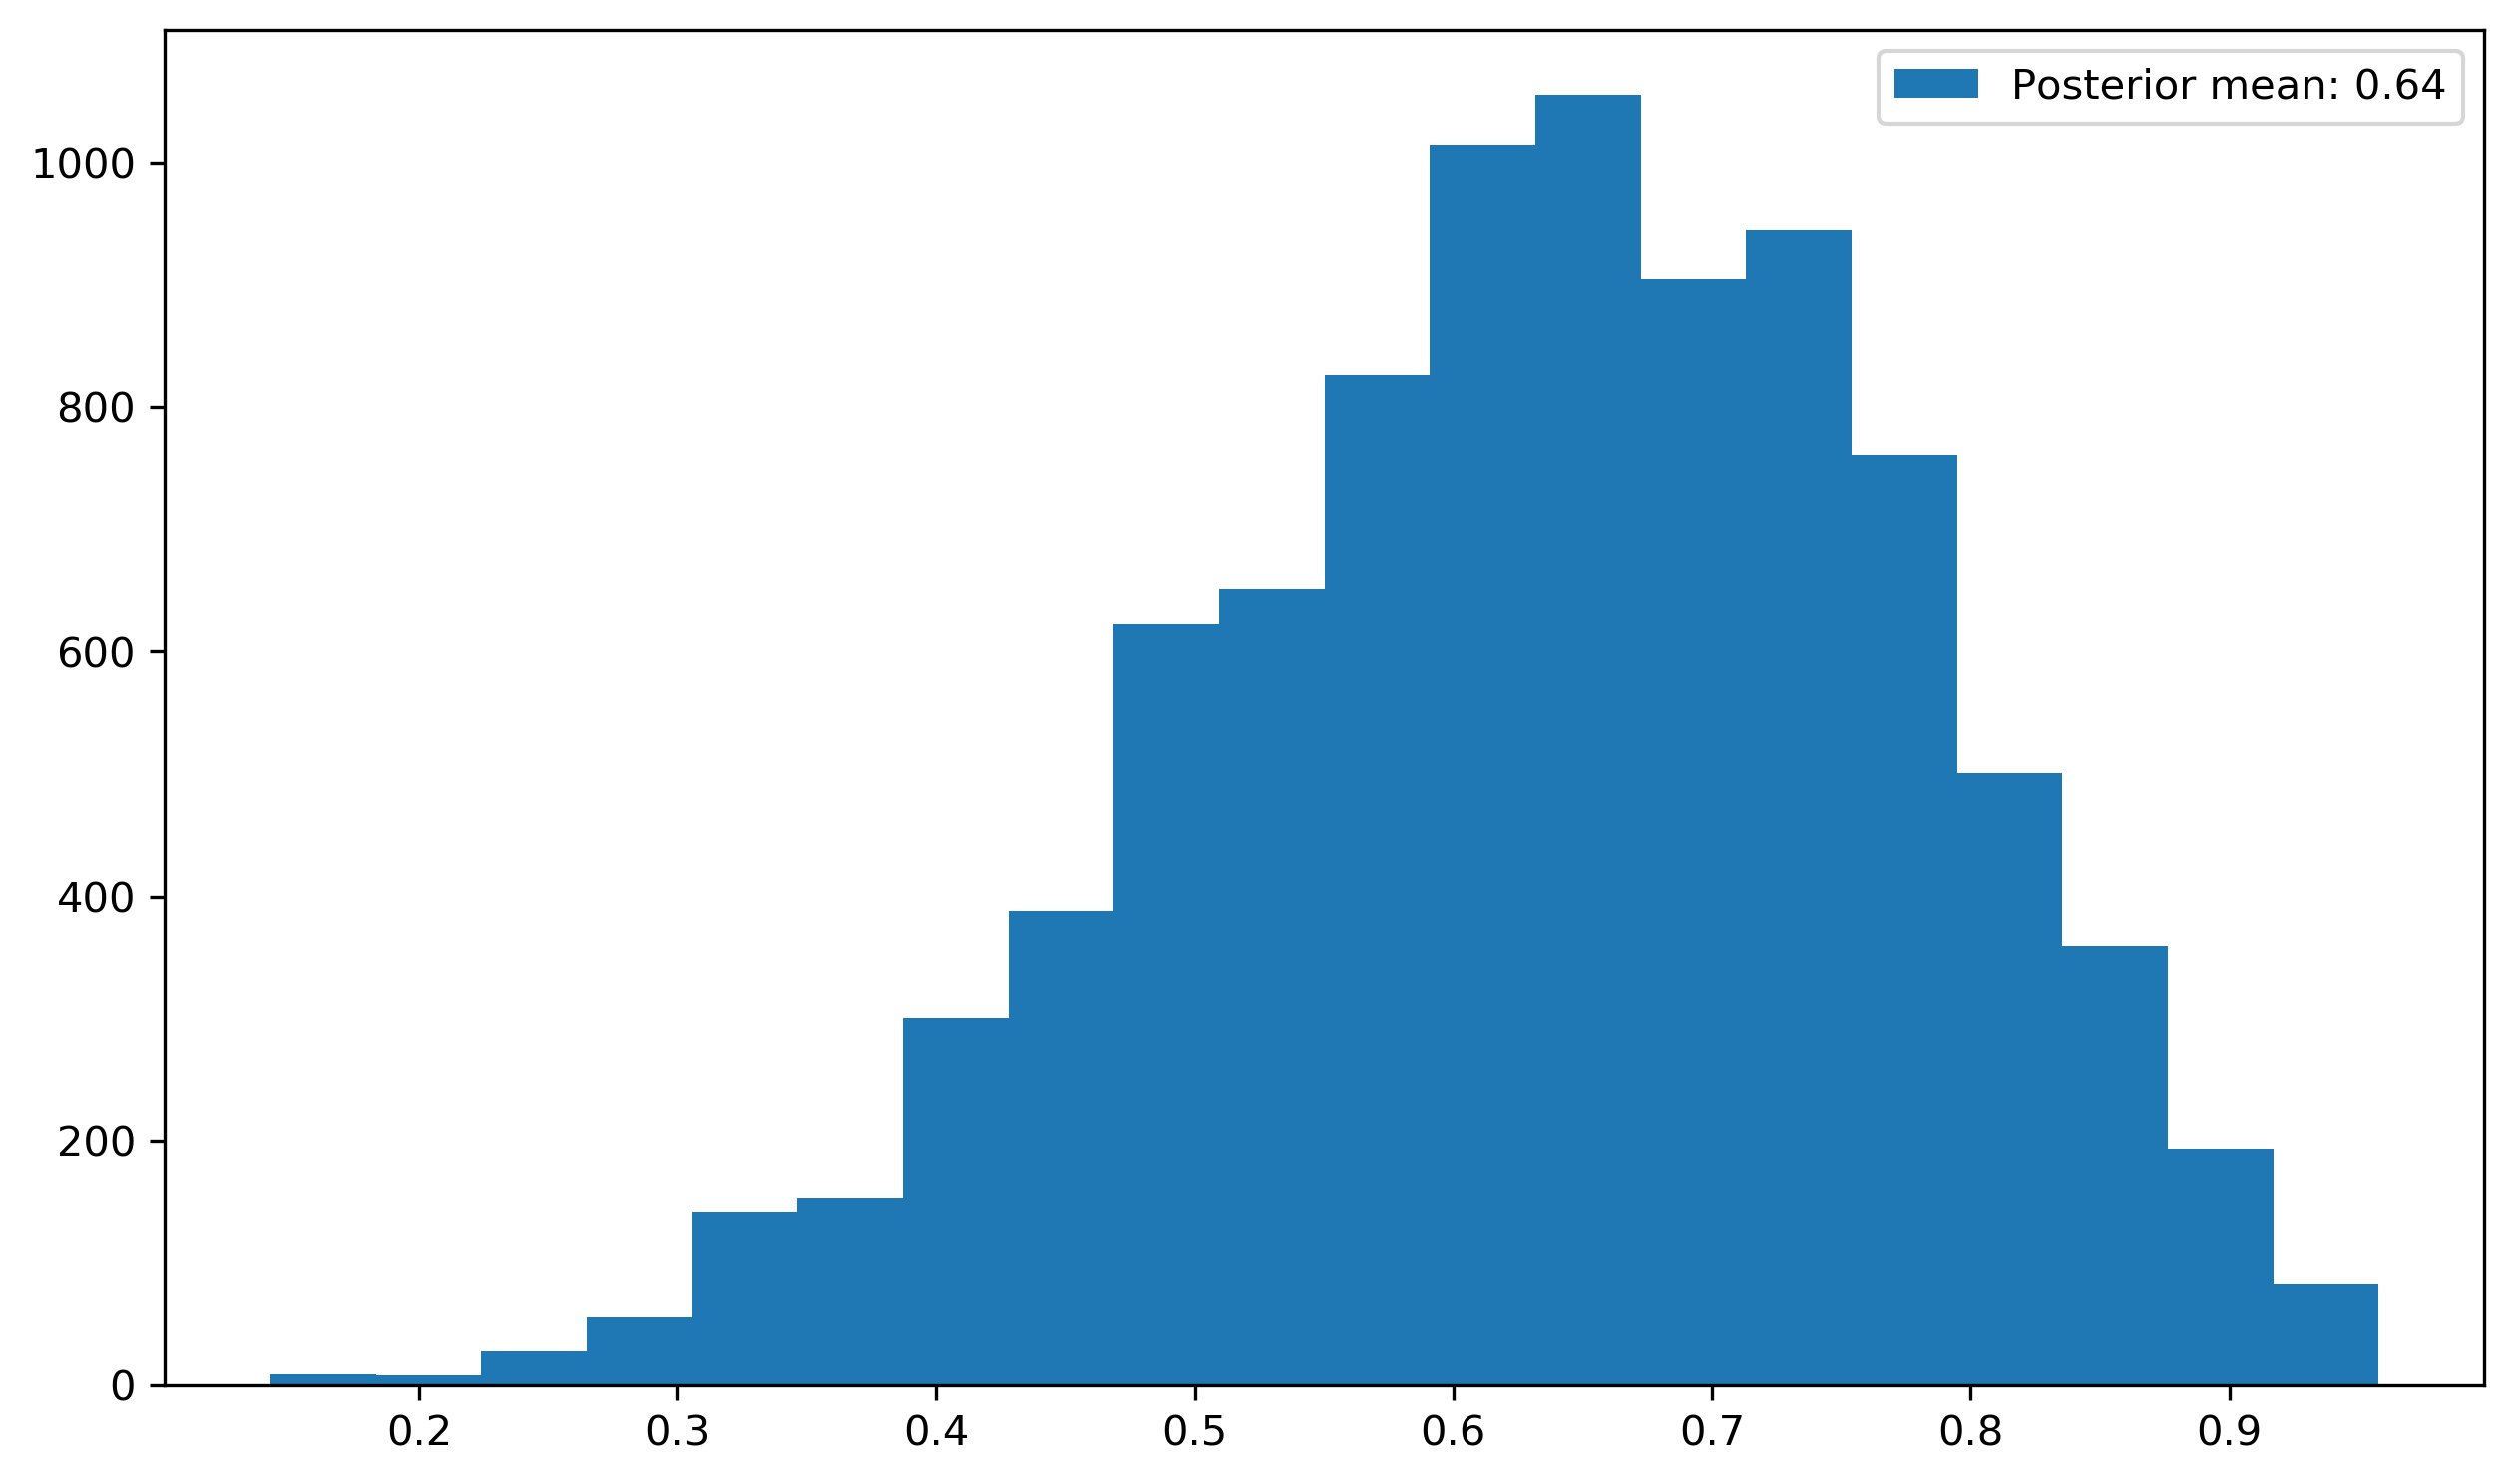
\includegraphics[width=.7\textwidth]{figs/metropolis.png}
\end{frame}

\begin{frame}[fragile]{Sampling algorithms}
	\begin{columns}
		\begin{column}{0.5\linewidth}
			\begin{easylist}[itemize]
				\ListProperties(Space=\listSpace, Margin1=1ex, Margin2=2ex, Space*=\listSpace, Style2*=$\color{bggraydark}\blacktriangleright$\space)
				# Many different sampling algorithms exist
				# Currently, the state-of-the-art is Hamiltonian Monte Carlo (HMC)
				## See e.g. Betancourt (2017): \footnotesize\texttt{https://arxiv.org/abs/1701.02434}
			\end{easylist}
		\end{column}
		\begin{column}{0.5\textwidth}
			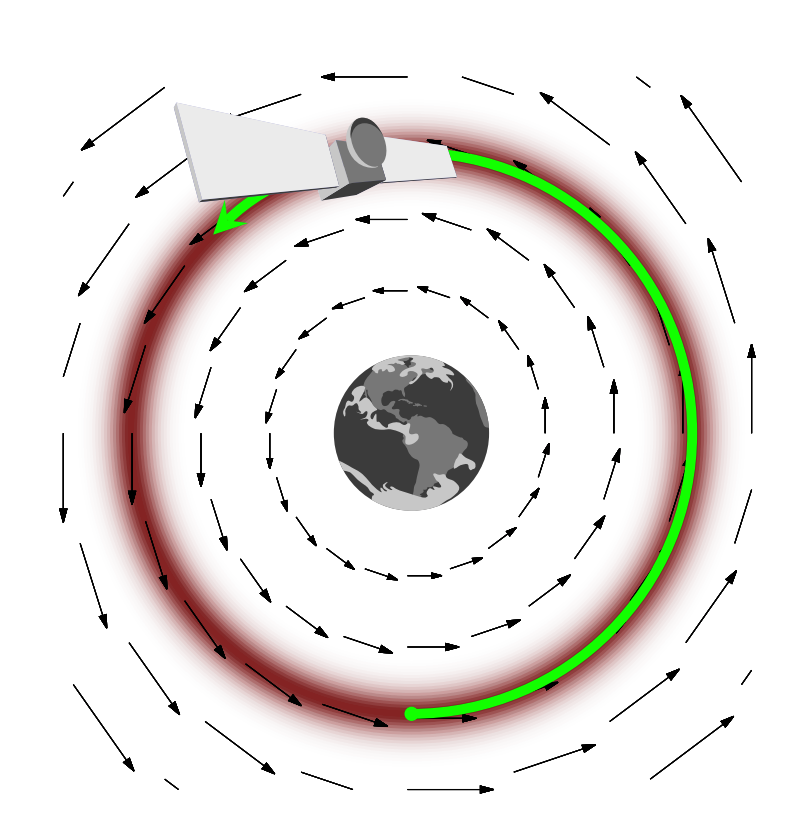
\includegraphics[width=\textwidth]{figs/hmc.png}
		\end{column}
	\end{columns}
\end{frame}

\begin{frame}[fragile]{Probabilistic programming in Python}
	\begin{columns}
		\begin{column}{0.5\linewidth}
			\begin{easylist}[itemize]
				\ListProperties(Space=\listSpace, Margin1=1ex, Margin2=2ex, Space*=\listSpace, Style2*=$\color{bggraydark}\blacktriangleright$\space)
				# PyStan
				# PyMC3
				# Pyro
				# TensorFlow Probability
			\end{easylist}
		\end{column}
		\begin{column}{0.5\textwidth}
			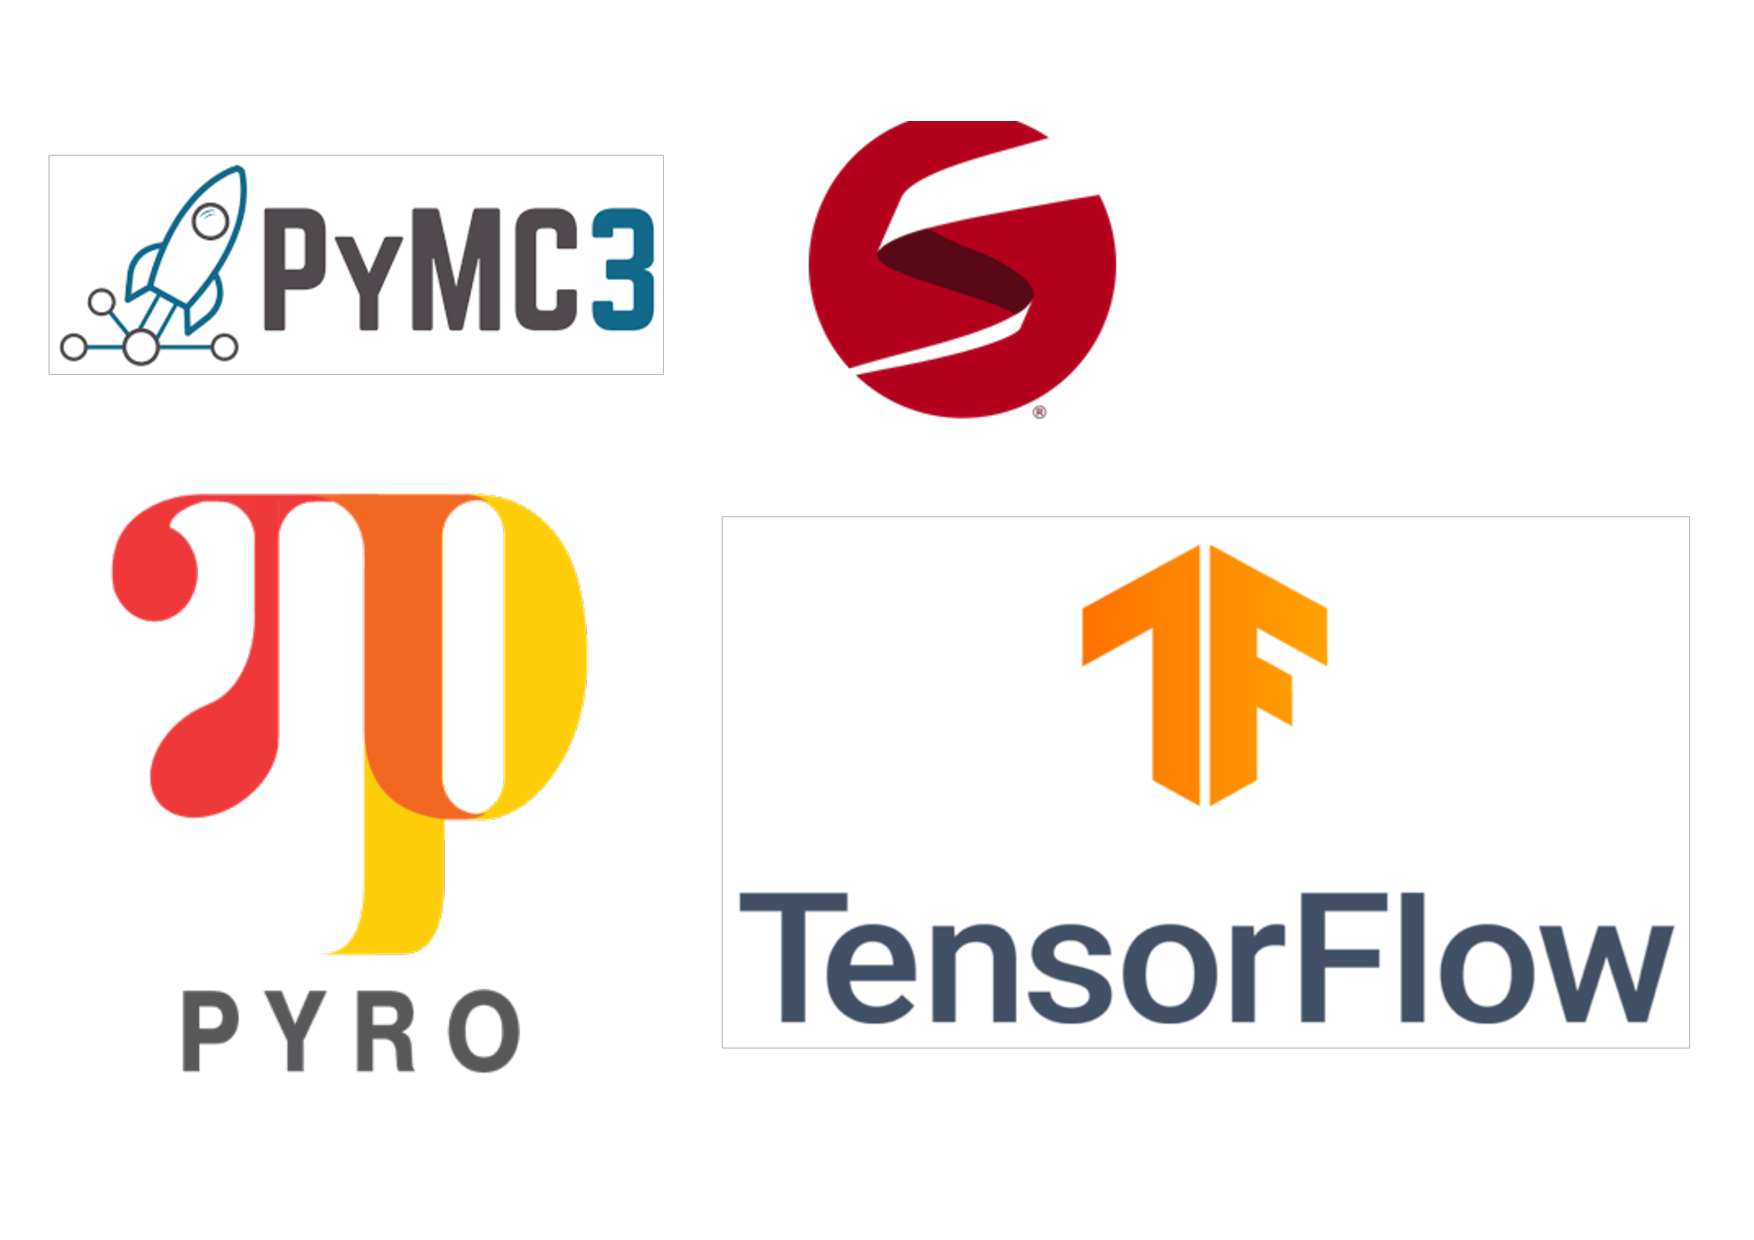
\includegraphics[width=\textwidth]{figs/logos.pdf}
		\end{column}
	\end{columns}
\end{frame}

\begin{frame}[fragile]{PyMC3}
	\begin{columns}
		\begin{column}{0.7\linewidth}
			\begin{easylist}
				\ListProperties(Space=\listSpace, Margin1=1ex, Margin2=2ex, Space*=\listSpace, Style2*=$\color{bggraydark}\blacktriangleright$\space)
				# Python package for for fitting Bayesian models using modern methods (MCMC, variational inference, etc.)
				# Well-documented, large suite of statistical models
				# Highly flexible, but easy to use
				# Uses Theano-backend (not good)
				# PyMC4 in development, uses TensorFlow Probability-backend
			\end{easylist}
		\end{column}
		\begin{column}{0.3\textwidth}
			
\includegraphics[width=\textwidth]{figs/pymc3.png}
		\end{column}
	\end{columns}
\end{frame}

\end{document}
